 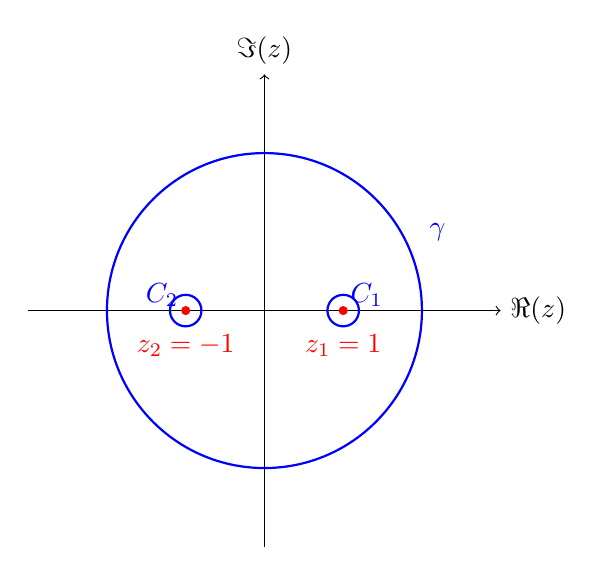
\begin{tikzpicture}[scale=1.0]
        % 画复平面
        \draw[->] (-3,0) -- (3,0) node[right] {$\Re(z)$};
        \draw[->] (0,-3) -- (0,3) node[above] {$\Im(z)$};
        
        % 画半径为2的圆
        \draw[blue, thick] (0,0) circle (2);
        \node[blue] at (2.2, 1) {$\gamma$};
        
        % 标出极点
        \filldraw[red] (1,0) circle (0.05) node[below=5pt] {$z_1=1$};
        \filldraw[red] (-1,0) circle (0.05) node[below=5pt] {$z_2=-1$};
        
        % 绘制绕过 z=1 的小圆弧（顺时针）
        \draw[blue, thick] (1,0) circle (0.2);
        \node[blue] at (1.3,0.2) {$C_1$};

        % 绘制绕过 z=-1 的小圆弧（顺时针）
        \draw[blue, thick] (-1,0) circle (0.2);
        \node[blue] at (-1.3,0.2) {$C_2$};
        
        % 指示方向
        % \draw[->, blue, thick] (1.5,0.5) -- (1.6,0.6);
    \end{tikzpicture}